\section{State of The Art}
\label{sec:int_state}

Solving the many-body problem remains one of the greatest challenges in physics.
Following the wealth of attempts at such pursuit, certain phenomena arising due to the strong interactions in quantum systems are explained in different theoretical frameworks, namely superconductivity, the Mott metal-insulator transition, and fractional quantum Hall effect.
All of these breakthroughs represented revolutions in their respective fields with significant scientific and technological impact.

Only in very limited cases does an actual analytical solution exist for the  Schr\"odinger equation for a system of interacting particles.
One must resort to sophisticated approximation methods to obtain  information about the role played by the competing interactions under various conditions in the aforementioned cases.
It is then natural that numerical methods have become prominent as a tool for extracting useful information about this type of systems.
\ac{QMC} is amongst the most accurate and extensively studied ones.

The idea of all \ac{QMC} methods is to reduce the interacting problem to solving a set of integrals, which can be evaluated numerically through a standard stochastic procedure.
These integrals are arrived at upon formulating the quantum many-body description of the system using the Schr\"odinger equation.
Hence the name \acl{QMC}, which is used to distinguish it from Classical Monte Carlo.
In the classical version, one measures thermal averages, while in the quantum version, one measures expectations of operators over the Hilbert space of the system, corresponding to physical observables that fluctuate with a dynamics given by the Schr\"odinger equation.

\subsection{Beyond graphene: TMD nanoribbons}

\ac{2D} materials have steadily been attracting more and more attention since graphene was experimentally isolated from a graphite sample by mechanical exfoliation, yielding a system constituted by a single layer of atoms (Figure \ref{fig:graphene}, left).
Since then, numerous studies have been made due to the promising properties of these materials, and the interesting as-yet-unseen phenomena occurring within them, for example: unconventional quantum Hall effect, absence of localization, and electrons behaving like massless relativistic particles (Figure \ref{fig:graphene}, right), providing a bridge between condensed matter physics and quantum electrodynamics \cite{katsnelson_graphene:_2007}.

\begin{figure}[H]
\hspace{1cm}
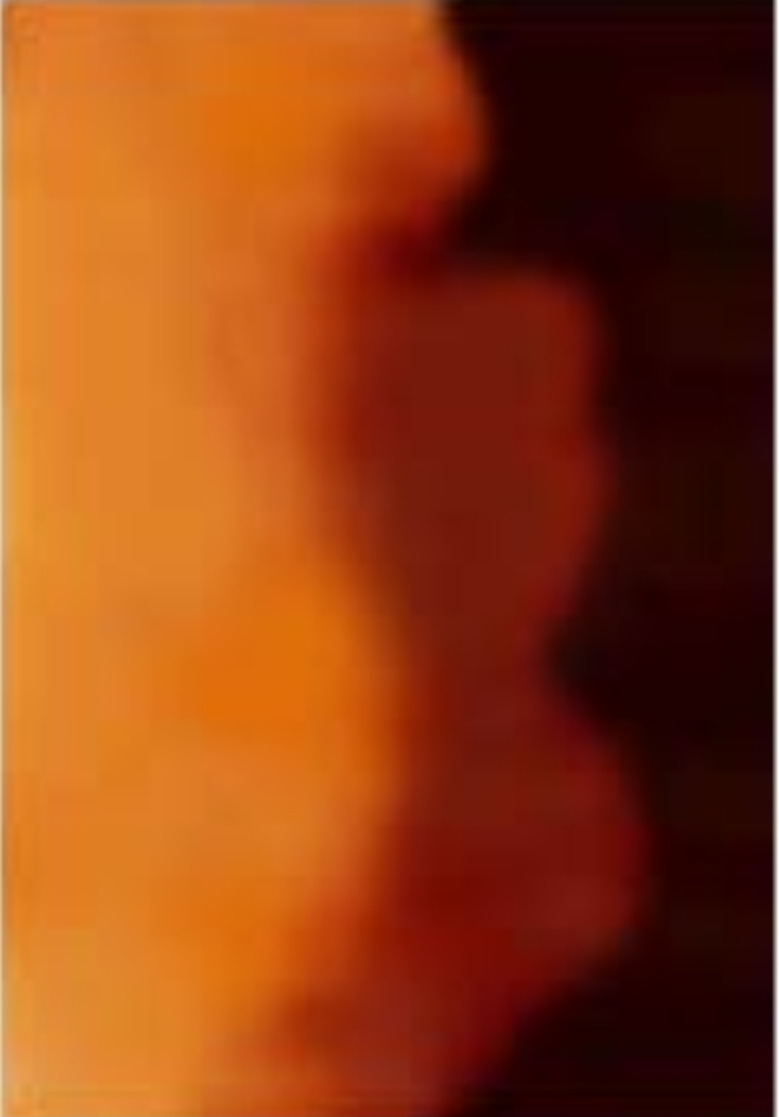
\includegraphics[width = 4.7cm]{Introduction/graphene.png}
\hspace{2cm}
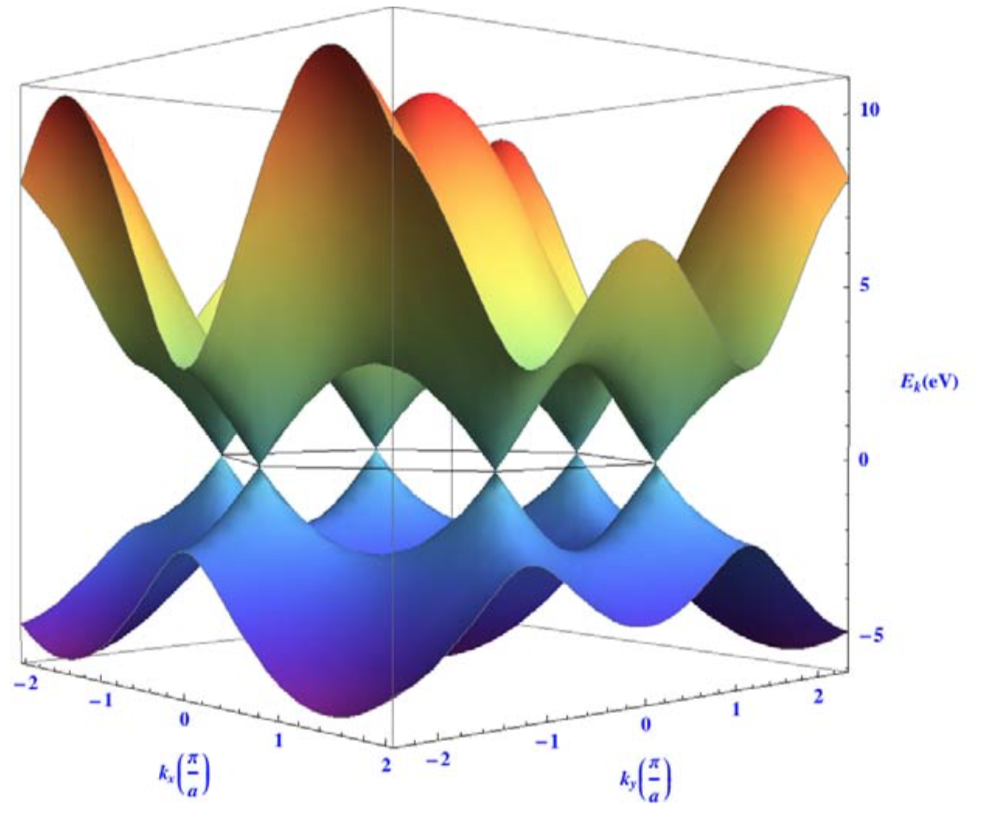
\includegraphics[width = 8.5cm]{Introduction/disp_rel.png}
\caption[Graphene monolayer; graphene's dispersion relation.]{Left: \acf{AFM} picture of a graphene monolayer. The black area is a substrate used for fabrication purposes. The dark orange area is a monolayer of graphene. Right: Dispersion relation of graphene. The black line represents the Fermi energy. Close to it, the dispersion relation is linear, corresponding to massless excitations (taken from \cite{noauthor_nobel_nodate}). }
\label{fig:graphene}
\end{figure}	

On the other hand, \acp{TMD} are a recent member of the \ac{2D} materials family \cite{wang_electronics_2012, roldan_electronic_2014, xu_spin_2014}.
\acp{TMD} have been attracting interest because they seem to overcome some of the drawbacks of graphene in technological applications.
For example, monolayer graphene is gapless, while its bilayer counterpart has only a tunable, but small gap of the order of a tenth of an $eV$.
Contrastingly, \acp{TMD} have an intrinsic gap in excess of $1 \, eV$, being more promising in designing, for example, transistors.
Hole-doped \acp{TMD} are expected to show topological superconductivity \cite{hsu_topological_2017}, while the superconducting phase of graphene has been predicted, but is not easily attained.
Superconductivity in graphene-like \ac{2D} materials is important because it could boost high speed nanoelectronics.
Moreover, the presence of transition metal atoms in \acp{TMD} suggests the possibility of magnetic ordering \cite{braz_valley_2017}, which could be very relevant in nanospintronics applications.
Both topological superconductivity and magnetic ordering arise due to the effect of strong electron correlations.
Thus, to investigate these properties of \acp{TMD} when performing simulations, we need a computational method that is robust enough to capture the effects of electron interactions.

A nanoribbon consists of a \ac{2D} layer that can be regarded as infinitely long on one direction, but not on the other (Figure \ref{fig:fabrication}), so that edge states become relevant, and can be controlled to yield interesting properties.
For simulation purposes, it is natural to assume translational invariance along the ribbon's longitudinal direction, and use \acp{PBC}.
On the other direction, we use \acp{OBC}, effectively considering zigzag edges (Figure \ref{fig:nanoribbons}, left).

\begin{figure}[H]
\centering
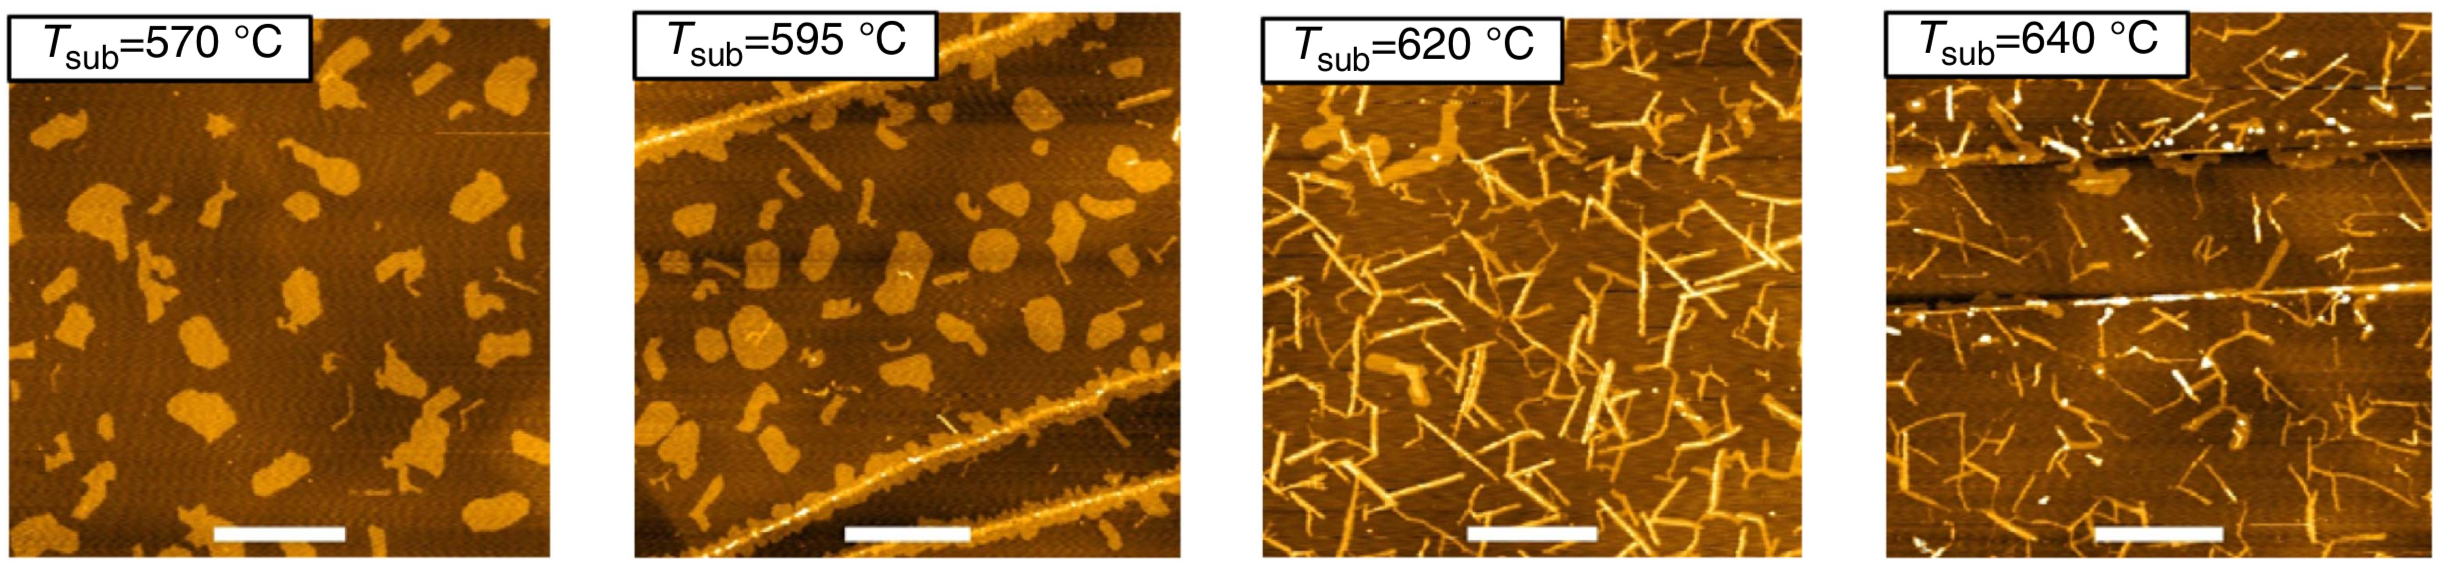
\includegraphics[scale = 0.35]{Introduction/nanoribbons}
\caption[Fabrication of \ac{TMD} nanoribbons]{Fabrication of \ac{TMD} nanoribbons. From left to right, we see \ac{AFM} images showing the appeareance of nanostructures ranging from \ac{2D} nanoislands to nanoribbons, as the temperature of the substrate is increased. The nanoribbons are grown by taking advantage of the temperature dependence of shape transformations occuring during the nonequilibrium growth of this kind of surface-based nanostructures. (taken from \cite{chen_fabrication_2017})}
\label{fig:fabrication}
\end{figure}
   
A high density of low-energy electronic states is localized at the zigzag edges, decaying quickly in the bulk, which suggests the possibility of magnetic ordering.
In fact, a mean field solution of the Hubbard model shows that magnetic moments are localized at the edges \cite{yazyev_emergence_2010} (Figure \ref{fig:nanoribbons}, right).
QMC has been used to investigate edge-state magnetism beyond mean field in graphene \cite{feldner_dynamical_2011, golor_quantum_2013, cheng_strain-induced_2015, raczkowski_interplay_2017, yang_strain-tuning_2017}.
However, edge magnetism in TMD nanoribbons remains unexplored \cite{davelou_nanoribbon_2017}.
 
\begin{figure}[H]
\hspace{2cm}
\begin{minipage}[c]{0.1\textwidth}
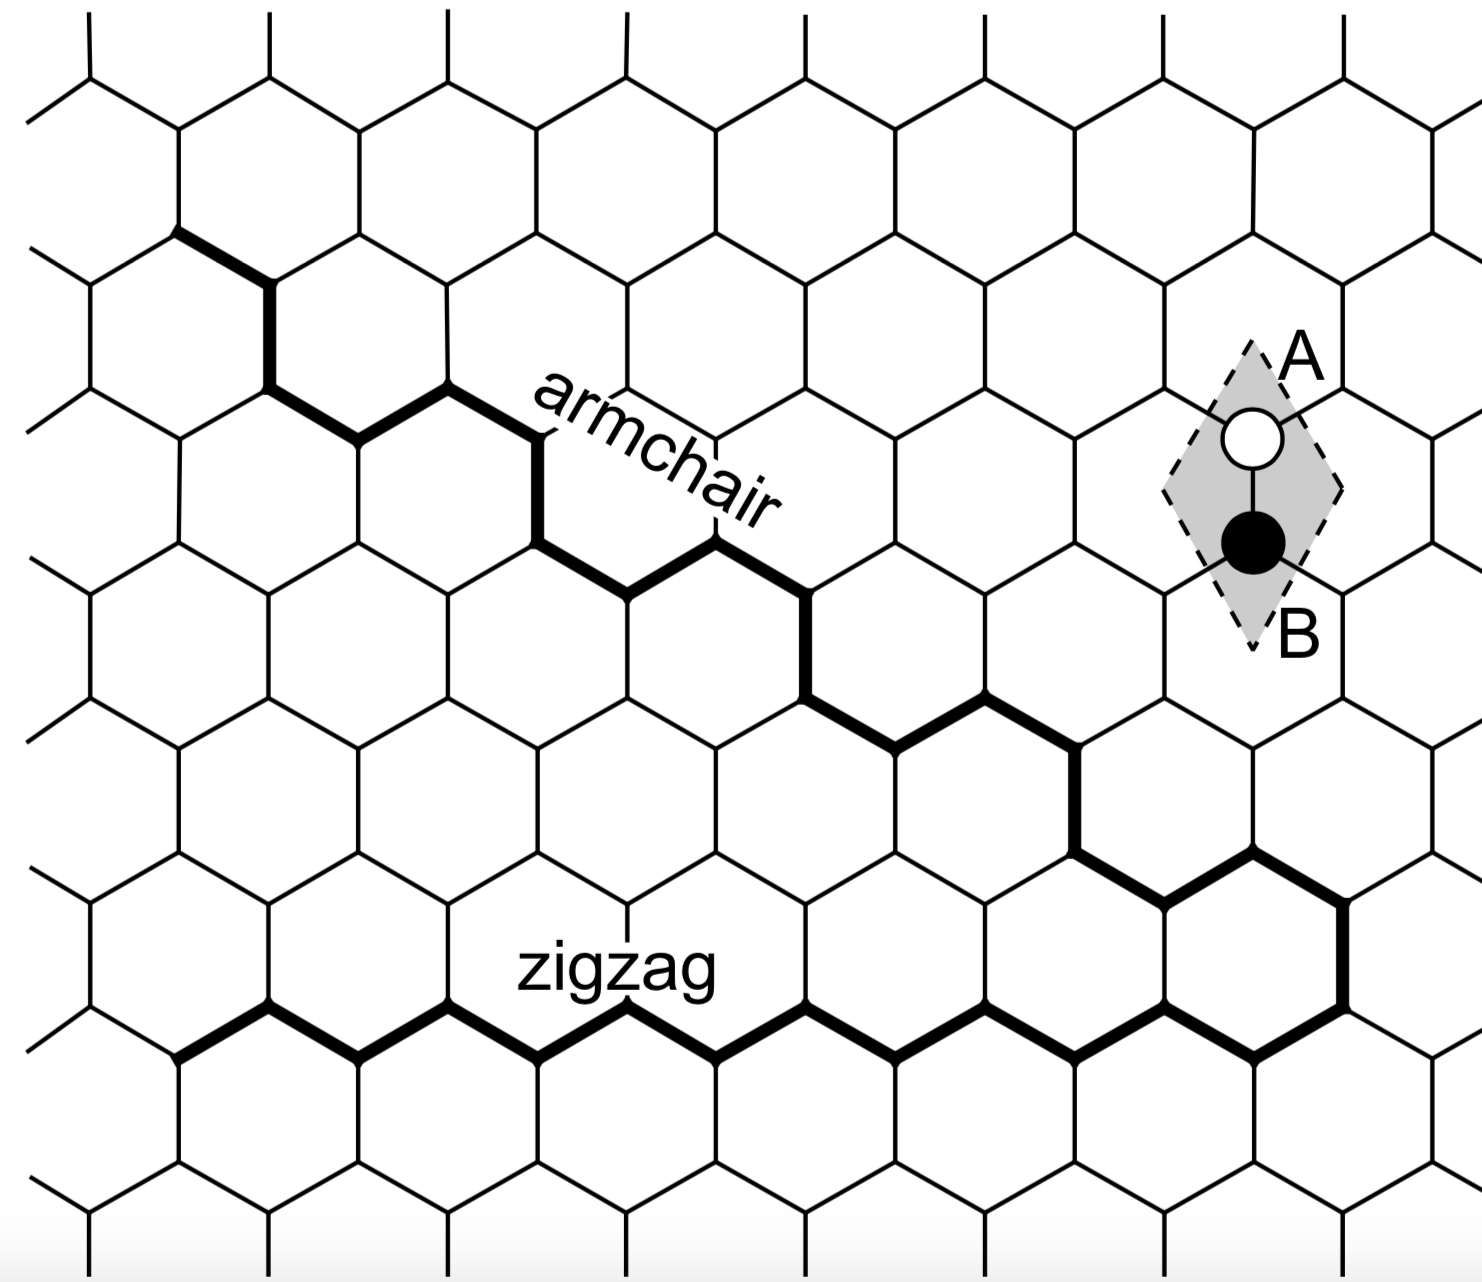
\includegraphics[scale = 0.22]{Introduction/zigzag}
\end{minipage} \hspace{6cm}
\begin{minipage}[c]{0.1\textwidth}
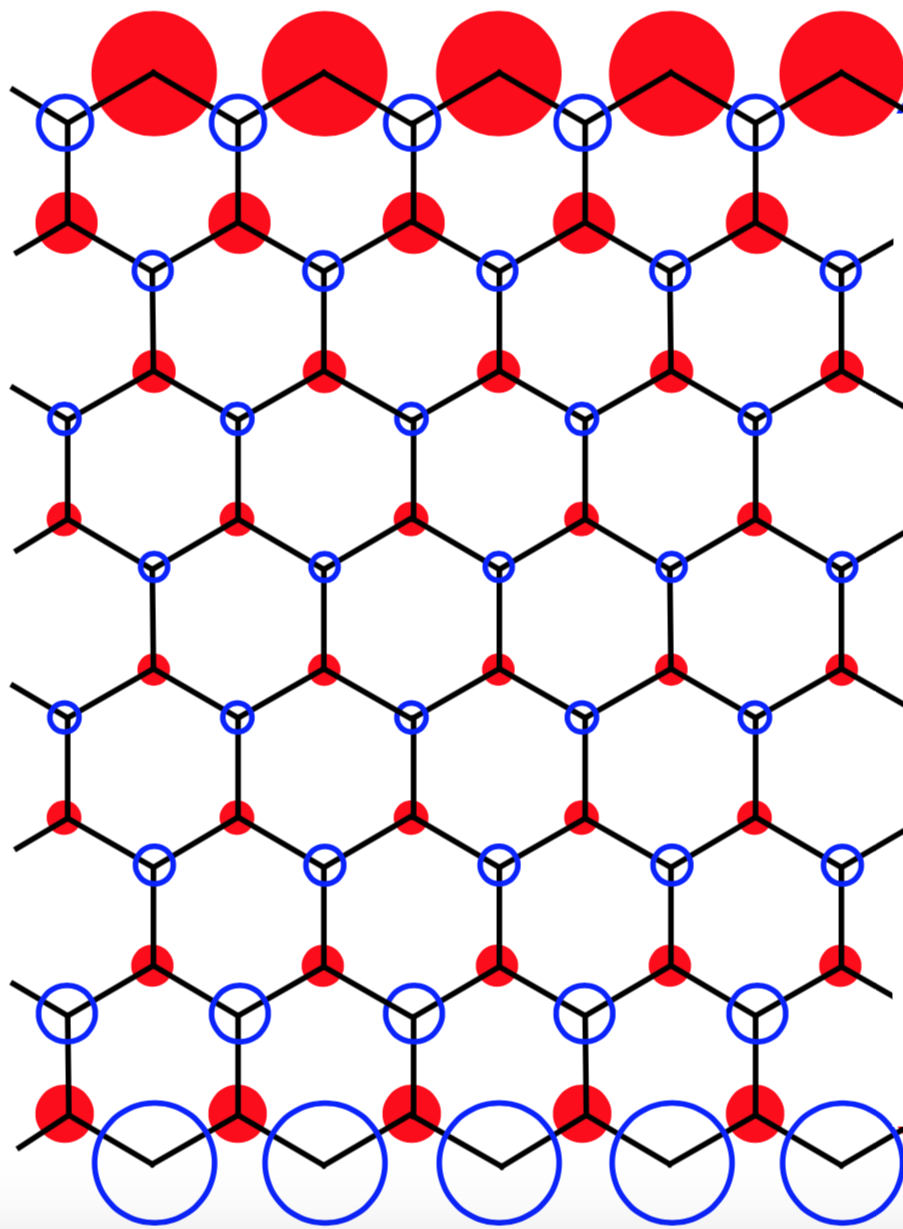
\includegraphics[scale = 0.23]{Introduction/edge_states}
\end{minipage}
 \caption[Zigzag edges of a nanoribbon and magnetism.]{Left: Two possible terminations of a \ac{TMD} nanoribbon condensing in a honeycomb lattice. Right: Local magnetic moments exist on the zig zag edges. The area of the circles corresponds to the magnitude of the magnetic moment, while the color red corresponds to a spin up density, and blue to a spin down density. The accumulation of $e^-$ edge states leads to an \ac{AF} ground state (opposite edges with opposite magnetic moment). (taken from \cite{yazyev_emergence_2010}) \label{fig:nanoribbons}}
\end{figure}

While the zigzag graphene nanoribbon antiferromagnetic ground state is semiconducting, a state with interedge ferromagnetic orientation is a metal.
An example of an application based on the switching between the two states is a magnetorresistive sensor.
This device allows switching between low and high-resistance configurations, corresponding, respectively, to parallel, and antiparallel configurations of ferromagnetic leads at the ends of a nanoribbon.
An important application of this project is precisely the investigation of the possibility of edge-state magnetism, as is observed in graphene nanoribbons, for TMD nanoribbons, which could yield similarly innovative applications.


\subsection{Introduction to \acl{QMC}}

In principle, the properties of a quantum many-fermion system can all be deduced by solving an extremely complicated Schr\"odinger equation that takes into account the coupling of all (identical) particles of the system.
However, for the majority of systems the resulting integrals have no analytic solution, so we solve the problem by numerical integration.
But there is a myriad of methods to evaluate integrals numerically.
How do we pick the best one for this case? 
It depends on the problem at hand, of course.
Variational and Diffusion \ac{QMC} are the simplest \ac{QMC} methods that allow one to capture some properties of correlated systems.
Although they already contain the main concepts used in this type of simulations, it is not always possible to use them. 
We will discuss their flaws and show how further refinement leads to the auxiliary field \ac{QMC} method.

A variety of \acf{QMC} methods exists, using a sampling scheme based on the Metropolis algorithm, and variations thereof.
However, applying them to many-fermion systems implies overcoming a significant obstacle common to all of them - the so called \emph{fermion-sign problem}.
Pauli's exclusion principle implies that the many-fermion wave function is antisymmetric, which leads to a sign oscillation that greatly impedes the accurate evaluation of averages.
Thus, a straightforward weight interpretation of the wave function is not possible.
In the case of the finite temperature algorithm, the cancellations that occur when computing the average of any physical observable lead to poor statistical properties of the estimators.
This means that a massive amount of measurements requiring enormous computer time are needed to obtain meaningful results.
In the case of the zero temperature algorithms, the situation is even worse.
It might not even be possible to design a stochastic process carrying the system to its ground state, as normally is done in \say{projective} methods\footnote{Methods that project a trial wave function onto the ground state.}: the wave function that is used as an initial proposal turns out to converge to a bosonic one, and the fermionic character of the system is lost.


As was proven by Troyer, the \emph{fermion-sign problem} has NP \footnote{NP or nondeterministic polynomial time roughly meaning that one can devise an algorithm that verifies the "yes" answer to a decision problem in polynomial time in the system size.
Note that the class $P$ - of polynomial time algorithms - is a subclass of NP.} computational complexity \cite{troyer_computational_2005}.
One of the greatest open questions in computer science is whether $P = NP$.
Solving the \emph{fermion-sign problem} would imply finding a solution to this problem, which would constitute a major breakthrough.

\subsection{Monte Carlo Method in  Classical Statistical Physics}

Monte Carlo methods form the largest and arguably most important class of numerical methods used to approach statistical physics problems. In these notes we explain what Monte Carlo techniques are and why they are useful. Statistical physics often deals with computing quantities that describe the behavior of condensed matter systems. The main difficulty one faces when doing so has to do with the collective nature of these systems. Many identical components comprise these systems, and while the equations that govern the behavior of the whole may be easy to write down, their solution is in general a remarkably laborious mathematical problem. The exponentially large number of configurations of a typical condensed matter system can be daunting. Analytical solutions are more often than not hopeless and even numerical solutions are seemingly challenging. However, they give valuable information lying between theory and experiment, and connecting them.

Suppose you try to sample uniformly from the probability distribution of all possible configurations of one of the aforementioned systems. Changes are your algorithm will not end before the Universe does. This is the computational complexity hurdle. A related issue is that of finite size effects. We are far from being able to simulate a macroscopically sized system. At best we can simulate a system that has only a minuscule fraction of the actual size of the corresponding real world system. Amazingly there are techniques that allow us to efficiently extract elusive information out of relatively small size simulations. Nonetheless, increasing the system size consistently improves the reliability of a simulation. Thus, the more efficient the algorithm is, the larger the system we can simulate in a fixed time.

The sheer number of equations describing a condensed matter system, and sometimes the strong coupling between them deems the task of finding an exact solution either very tough or even impossible. It is not even clear whether an analytical solution would be of any use in many cases, and a statistical and numerical treatment often allows us to study more effectively the key properties of a system. Analytical solutions are rare. Exact solutions are an even rarer accomplishment. Not only do analytical solutions rely on approximations, but also numerical methods.

On the other hand, let us emphasize the striking victory of statistical mechanics. We are able to describe a system that is governed by a macroscopically large number of equations in terms of only a few variables. The loss of information in doing so is only apparent. The statistical description is so effective because most of the possible states of the system are extremely improbable when compared to the relevant very narrow part of configuration space. The success of the field is largely attributed to the averaging out that naturally occurs when we measured a property of a macroscopic system.

How do we set up a simulation of a physical system? We assume basic knowledge of statistical physics and focus only on the concepts that are essential for simulation purposes.

A system in state $\mu$ makes transitions to state $\nu$ at a rate $R(\mu \rightarrow \nu)$


The Monte Carlo method is ubiquitous. Its central idea is to use randomness to produce accurate estimates of deterministic integrals. The term was coined by Nicolas Metropolis in 1949, first appearing in a seminal paper, in which it was described as a \say{statistical approach to the study of differential equations, or more generally, of integro-differential equations that occur in various branches of sciences}\cite{Metropolis1949}. Although it was used as early as 1777 in an experiment known as Buffon's needle - where one obtains an estimate of the constant $\pi$ by repeatedly throwing  a needle randomly onto a sheet of paper with evenly spaced lines - it was crucially developed in the Los Alamos National Laboratory during World War II where the development of the first atomic bomb was completed, the primary objective of the Manhattan Project. The method is particularly useful when one wants to sample from a probability distribution in an exponentially large state space. In fact, it can in principle be used to solve any problem allowing a probabilistic formulation.

The law of large numbers affords an approximation to integrals which can be written as an expectation of a random variable. Upon drawing enough independent samples from the corresponding distribution, the sample mean gets arbitrarily close to the integral at stake.

\begin{equation}\label{eq:int_mean}
\mathbb{E} [f(X)] = \int dx f(x) p(x),
\end{equation}
where $p(x)$ is the distribution of $X$. 

We could simply draw $M$ independent and identically distributed samples $x_{1,...M}$ from $p(x)$ and approximate the integral as

\begin{equation}
\frac{1}{M} \sum_{k=1}^M f (x_k) , 
\end{equation}
which in most cases converges to the desired expectation, as long as $M$ is large enough. How large?

\begin{equation}\label{eq:variance}
\text{Var}\bigg( \frac{1}{M} \sum_{k=1}^M f(x_k) \bigg) = \frac{1}{M} \text{Var}\bigg( f(x_1) \bigg) \sim \mathcal{O}\bigg(\frac{1}{M}\bigg)
\end{equation}

Thus, the correction to the sample mean is of order $\mathcal{O}(M^{-1/2})$.

How do we sample from an arbitrary distribution $p(X)$? The idea is to first make an educated choice of a Markov Chain with the prescribed stationary distribution from which we ultimately desire to sample from, $p(X)$. After a sufficiently high number of steps, a Markov Chain Monte Carlo (MCMC) algorithm generates samples from the target distribution. Imposing some conditions on this Markov Chain, namely that it should be irreducible, aperiodic and positive recurrent, the ergodic theorem guarantees that the empirical measures of the aforementioned sampler approach the target stationary distribution. Another important condition to impose on this Markov Chain is detailed balance. Let the transition matrix be $\bm P = [p_{ij}]$, and the state space $\Omega$ be $\{\pi_i | i=1, ..., |\Omega| \}$, where $|\Omega|$ is the total number of possible states. Then, the condition of detailed balance is defined for all $i, j$ as

\begin{equation}
\pi_i p_{ij} = p_{ji} \pi_j 
\end{equation}

Crucially, Monte Carlo methods employ \emph{importance sampling}. It turns out that we can improve upon our estimate of $\mathbb{E} [f(X)]$ by introducing a separate distribution $q(x)$, and defining the weight function as $w(x) = p(x)/ q(x)$. Then, we can rewrite equation (\ref{eq:int_mean}):

\begin{equation}
\mathbb{E} [f(X)] = \int dx f(x) q(x) w(x) = \mathbb{E} [f(Y) w(Y)],
\end{equation}
with $Y \sim q$, i.e. the random variable $Y$ follows the distribution $q(Y)$

It appears as though we didn't gain anything. However, by choosing $q$ wisely, we can actually reduce the variance we computed in equation (\ref{eq:variance}):

\begin{equation}
\text{Var}\bigg( \frac{1}{M} \sum_{k=1}^M f(y_k) w(y_k) \bigg) = \frac{1}{M} \text{Var}\bigg( f(y_1) w(y_1) \bigg)
\end{equation}

Since we didn't make any assumptions about $q(Y)$, it may be chosen so as to minimize the variance, hence the error of the Monte Carlo estimator, improving the approximation of the expectation. However, note that the error remains of order $\mathcal{O}\big(\frac{1}{\sqrt{M}}\big)$.

The idea of the Quantum (Classical) Monte Carlo method is to simulate the random quantum (thermal) fluctuations of the system, as it oscillates between states in a given time frame \cite{Newman1999}. Instead of visiting these states uniformly, the algorithm applies \emph{importance sampling}: the most relevant part of the phase space is sampled more frequently, overcoming the seemingly exponential complexity of computing a sample mean numerically. Even though only a small fraction of the system's states are sampled, we obtain an accurate estimate of physical quantities of interest, namely energy, and correlation functions.

QMC generally provides an accurate approximation of the solution to the quantum many-body problem. When relativistic effects are negligible, which is the case of most condensed matter systems, any physical system can be described by a many-body Schr\"odinger equation. The issue is that the many-body wave function lives in the corresponding Hilbert space that is  exponentially large in the number of particles. For example, the number of possible states of a physical system whose configuration space rests on a two-dimensional lattice is exponentially large. The method described above is applied to approximate the multidimensional integrals arising upon formulating the quantum many-body problem in this space.

One can set up a na\"ive mean field theory in which the many body wave function is approximated by an antisymmetric function of one body wave functions\footnote{This corresponds to the Hartree-Fock approximation that we used to derive the Hubbard Hamiltonian in section \ref{hubbardHamiltonian}.}. One of the drawbacks of this approach is that the effect of  correlations is not captured. Fermionic QMC goes beyond mean field theory,  capturing the phenomena occuring within strongly correlated electronic systems. For non-frustrated boson systems, a polynomially scaling algorithm leads to an exact solution. For a fermionic system, such as the TMD nanoribbon, the existing algorithms usually provide accurate yet not exact solutions, which would in general require exponential computing time. This is due to the so called sign problem. We will discuss this numerical issue later.

\section{Variational Monte Carlo}

Variational techniques rely on an educated guess for the wave function of the system. One often introduces a set of variational parameters $\bm \alpha$ that are then tuned according to a variational principle. We use the optimized trial wave function to compute physical quantities of interest using Monte Carlo. Note that the method requires  prior knowledge about the system. We will see that it is natural to combine the Metropolis algorithm for quantum many-body systems with the variational principle.

A particularly relevant observable is the variational energy $E_V$ associated with a given quantum state. Let $\bm r$ be the $3N$ spatial coordinates of the $N$ electrons. Given the Hamiltonian of the system $\mathcal{H}$, and a trial wave function $\psi (\bm r)$ - hopefully a good guess of the wave function representing some state of the system - one can compute the variational energy.

\begin{equation}\label{eq:variational_energy}
E_V = \frac{\left\langle \psi | \mathcal{H} | \psi \right \rangle}{\left\langle \psi | \psi \right \rangle} = \frac{ \int d\bm r |\psi (\bm r)|^2 E_L (\bm r)}{\int d\bm r | \psi (\bm r)|^2 } = \int d\bm r\rho (\bm r) E_L (\bm r) ,
\end{equation}
where the local energy $E_L (\bm r)$ is defined as

\begin{equation}\label{eq:local_energy}
E_L = \frac{\mathcal{H} \psi (\bm r) }{\psi (\bm r)}
\end{equation}
and the probability distribution $\rho (\bm r)$ is defined as

\begin{equation}\label{eq:rho}
\rho (\bm r) = \frac{ | \psi (\bm r) |^2}{ \int d\bm r' | \psi (\bm r') |^2}
\end{equation}

Note that we managed to recast the variational energy as an average  of the \emph{local} energy, $< E_L > $, over the the distribution $\rho$. This is easily estimated by sampling $M$ points $\bm r_k$ from $\rho (\bm r)$:

\begin{equation}\label{eq:average}
E_V \approx \overline E_L = \frac{1}{M} \sum_{k= 1}^{M} E_L (\bm r_k) ,
\end{equation}
where $\overline {X}$ denotes a sample mean of the random variable $X$. A common sampling scheme is the Metropolis-Hastings algorithm.

How do we optimize a variational state? Suppose we are particularly interested in the ground state energy $E_0$. Then, the variational principle reads

\begin{equation}
E_{0_V}[\alpha_i] = \frac{< \psi_0 | \mathcal{H} | \psi_0 >}{<\psi_0 | \psi_0>} \ge E_0,
\end{equation}
where $\psi_0$ is the ground state wave function. By varying $\alpha$ we aim to obtain a variational energy that is as close as possible to the true ground state energy. Since $E_{0_V}(\alpha)$ is bounded from below, this is equivalent to minimizing it in the hope that $E_{0_V}(\alpha_{min}) \gtrsim E_0$ 

The use of an approximate wave function introduces a systematic error. The finite sampling size $M$, however, introduces a statistical uncertainty common to all Monte Carlo methods. 

\subsection{Variational Techniques}

It is natural to combine the Metropolis algorithm for quantum many-body systems with a variational principle. The goal is to find a variational wave function which can be optimized so that ultimately we obtain as accurate as possible an estimate of the ground state of the system \cite{tao}.\par

The parameters $\bm \alpha$ of a trial wave function $\phi(\bm r)$ are optimized according to the variational principle

\begin{equation}
E[\alpha_i] = \frac{< \phi | \mathcal{H} | \phi >}{<\phi | \phi>} \ge E_0,
\end{equation}
where $E_0$ is the ground state energy.

In fact, expanding in terms of the eigenstates of the hamiltonian $\{ \psi_n (\bm r) \}$, a complete basis set:

\begin{equation}
\phi (\bm r) = \sum_{n= 0}^{\infty} a_n \psi_n (\bm r) ,
\end{equation}
and plugging it back into the variational principle, subject to $E_n \ge E_0 ,\, n > 0$ and $<\psi_n | \psi_m> = \delta_{nm}$ we obtain

\begin{equation}
E[\alpha_i] = \frac{\sum_n a_n^2 E_n}{\sum_n a_n^2 } \ge E_0
\end{equation}

The expectation is the integral

\begin{equation}
E[\alpha_i] = \frac{\int \phi^\star (\bm r) \mathcal{H} \phi (\bm r) d\bm r}{\int | \phi (\bm r') |^2 d\bm r'} \equiv \int W(\bm r) E(\bm r) d\bm r ,
\end{equation}
where the integrand is a quantity which may be regarded as a distribution function $W(\bm r) = \frac{|\phi (\bm r)|^2}{\int |\phi(\bm r')|^2 d\bm r'}$ and a local energy of the system at configuration $\bm r$: $E(\bm r) = \frac{\mathcal{H}\phi(\bm r)}{\phi (\bm r)}$.

Given $W(\bm r)$ and $E(\bm r)$, one can in principle evaluate $E[\alpha_i]$. In practice $\phi (\bm r) $ is parametrized depending on the physical model at play, and the variational parameters $\alpha_i$ in the trial wave function are optimized by minimizing $E[\alpha_i]$.\par

The Metropolis algorithm is used to sample a set of points $\{\bm r_i\}$ from the configuration space, and the evaluation of the expectation value $E[\alpha_i]$ in each QMC step for each set of variational parameters is the equivalent of computing an average of a classical quantity at a given temperature in classical Monte Carlo. Systematically, we optimize the wave function based on the Euler-Lagrange equation

\begin{equation}
\frac{\delta E[\alpha_i]}{\delta \alpha_j} = 0
\end{equation}

An example of a thorough discussion on the systematic procedure to do this is given in \cite{umrigar}.\par

An important aspect of the variational wave function - hopefully an already  reasonable approximation of the ground state - is that it should be stable when two particles approach each other and the interaction diverges. This divergence is commonly canceled by their relative kinetic energy when their separation goes to zero - \emph{cusp condition}\cite{mahan}. Building this condition into the variational wave function significantly reduces fluctuations in the results, yielding larger accuracy when dealing with systems with a larger number of particles.


\subsection{Diffusion Monte Carlo}\label{subsec:dmc}

Variational Monte Carlo is limited by the use of a trial wave function $\phi (\bm r)$: we may not have enough information to even construct a reliable variational wave function in the first place. \cite{tao}\par

Diffusion QMC allows the simulation of a many-body system while having only a limited knowledge of the system's physical properties. While it is exact for many-boson systems, it is only approximate for many-fermion systems. The idea is to map the Schr\"odinger equation into  an imaginary-time diffusion equation. Excited states are then filtered out by a diffusion process as time passes. In imaginary-time $\tau = - i t$, the solution to Schr\"odinger's equation in terms of a formal series expansion in the eigenfunctions of the hamiltonian becomes a series of transients $e^{-E_n \tau}, \, n \in \mathbb{N}$. The longest lasting of these is the ground state. \cite{kosztin} \par

The idea of DQMC is to generate samples using the exact ground state wave function $\phi_0 (\bm r)$ \cite{vmc}. The associated exact energy $E_0$ is the matrix element of the hamiltonian calculated using a trial wave function and the ground state wave function.

\begin{equation}
\begin{split}
&E_0 = \frac{ < \phi_0 |E_0 \mathbbm{1} | \phi >}{< \phi_0 | \phi >} = \\
&= \frac{< \phi_0 | \mathcal{H} | \phi >}{ <\phi_0 | \phi >} = \frac{\int d\bm r \phi_0^\star (\bm r) \phi (\bm r) E_L (\bm r)}{\int d\bm r\phi_0^\star (\bm r) \phi (\bm r)}
\end{split}
\end{equation}

Note that using this trick we avoid the computation of $\mathcal{H} \phi_0 = E_0 \phi_0$, that is, the ground state energy. Instead, we approximate the integral by considering $N$ configuration samples $\bm r_{k = 1,..., N}$ in a similar spirit to that of VQMC. Notice that the integral consists of a local energy of the trial wave function $E_L (\bm r) = \frac{\mathcal{H} \phi (\bm r)}{\phi (\bm r)}$ averaged over a mixed distribution from which we draw a sample of points $\bm r_{k=1,...N}$.

\begin{equation}
f(\bm r) = \frac{\phi_0^\star (\bm r) \phi (\bm r) }{ \int d\bm r  \phi_0 (\bm r) \phi (\bm r)}
\end{equation}

Take a single particle in 1D. Performing a Wick rotation - effectively going to imaginary time - and shifting the energy, Schr\"odinger's equation becomes

\begin{equation}
\partial_\tau \psi = -\frac{1}{2m} \partial^2_x \psi - \bigg[ V(x) - E_T \bigg] \psi
\end{equation}

The exact ground state wave function $\phi_0$ is obtained as the longest lasting transient state in imaginary time; we are interested in the asymptotic behavior of the series expansion constituting the formal solution of Schr\"odinger's equation

\begin{equation}
\psi (x, \tau) = \sum_{n=0}^{\infty} c_n \Phi_n (x) e^{-(E_n - E_T)\tau}
\end{equation}

Imaginary time evolution is governed by

\begin{equation}\label{eq:im_ev}
\begin{split}
&| \psi (t) > = \lim_{\tau \rightarrow \infty} \sum_i e^{-(E_i - E_T) \tau} |\psi_i > <\psi_i | \psi > = \\
&= \lim_{\tau \rightarrow \infty} e^{-(E_0 - E_T)\tau} | \phi_0 >< \phi_0 | \psi > 
\end{split}
\end{equation}


If $E_T > E_0$ the wave function diverges exponentially fast: $\lim_{\tau \rightarrow \infty} \psi ( x, \tau) = \infty$. Similarly, for $E_T < E_0$ it vanishes exponentially fast: $
\lim_{\tau \rightarrow \infty} \psi ( x, \tau) = 0$. However, if $E_T = E_0$ the wave function converges to the ground state one up to a constant factor.

\begin{equation}\label{eq:dmc}
\lim_{\tau \rightarrow \infty} \psi ( x, \tau) = c_0 \phi_0 (x) \,\,\, \text{, or} \quad \lim_{\tau \rightarrow \infty} |\psi (\tau) > \propto | \phi_0 >
\end{equation}

DQMC makes use of equation (\ref{eq:dmc}), approximating $\phi_0(x)$ by $\psi (x, \tau)$ for sufficiently long time. The only requirement is that $\psi (x, \tau)$ and $\phi_0(x)$ overlap significantly so that $c_0$ is large enough to be numerically measurable, and we can always center a positive trial wave function in a region where $\phi_0(x)$ is large enough. This is always possible for a single particle,  but note that it might fail for a many-fermion system for which the wave function crosses a number of nodes due to its antisymmetric nature.\par

\subsection{Path Integral Formulation}\paragraph{}

In position representation, we may rewrite equation (\ref{eq:im_ev}) by noting that

\begin{equation}\label{eq:green}
\psi(\bm r_f, \tau) = \int d\bm r_i G( \bm r_f | \bm r_i ; \tau) \psi (\bm r_i) ,
\end{equation}
where we have defined the Green function $G( \bm r_f | \bm r_i ; \tau) \equiv < \bm r_f | e^{-(\mathcal{H} - E_T) \tau} | \bm r_i >$, the imaginary-time propagator. This allows for a path integral interpretation of the diffusion method. Take equation (\ref{eq:green}), multiply by $\psi (\bm r_f)$ and divide by $\psi (\bm r_i)$ to obtain the evolution equation for the mixed distribution $f(\bm r, t) = \psi (\bm r, \tau) \psi (\bm r)$:

\begin{equation}
f(\bm r_f, \tau) = \int d\bm r_i \tilde{G} ( \bm r_f | \bm r_i; \tau) \psi (\bm r_i)^2 ,
\end{equation}
where we have redefined an \emph{importance sampling} Green function $\tilde{G} (\bm r_f | \bm r_i; \tau) = \psi (\bm r_f) G(\bm r_f | \bm r_i ; \tau) \frac{1}{\psi(\bm r_i)}$. 

The mixed distribution approaches the target stationary distribution: $f(\bm r) = \lim_{t\rightarrow \infty} f(\bm r, t) \propto \phi_0(\bm r) \psi (\bm r) $

In the limit of short propagation time, the action of the $\hat T$ and $\hat V$, the kinetic and potential energy operators, does not significantly change the states acted upon separated by the short interval $t$: $| \chi (t') >$ and $|\chi (t'+t) >$. Furthermore, one can use the Trotter-Suzuki decomposition, based on the result that for a - not necessarily commuting - set of operators $\{A_i | \, i = 1,...p\}$  we can write

\begin{equation}
e^{A_1 + A_2 + ... + A_p} = \lim_{m\rightarrow \infty} ( e^{A_1/m}e^{A_2/m}...e^{A_p/m})^m
\end{equation}

In this case it allows us to rewrite $e^{-(\hat T + \hat V) t} = e^{-\hat V t/2} e^{-\hat T t} e^{-\hat V t/2} + \mathcal{O}(t^3) $. Further acting with the potential operator on the left and on the right, we find an analytical expression for the propagator.

\begin{equation}
G(\bm r_f | \bm r_i ; \tau) \approx \frac{e^{-\frac{(\bm r_f - \bm r_i)^2}{2t} -\big( \frac{V(\bm r_f) + V(\bm r_i)}{2} - E_T \big) t}}{(2\pi t)^{3N/2}} 
\end{equation}

The \emph{fermion sign problem} will shortly become apparent. The key assumption that breaks for many-fermion wave functions is that the trial wave function does not change sign so that $\psi (\bm r_f) / \psi (\bm r_i) > 0$. In the latter case, the short time \emph{importance sampling} Green function becomes

\begin{equation}
\begin{split}
\tilde{G}(\bm r_f | \bm r_i ; \tau) \approx & \frac{1}{(2\pi t)^{3N/2}} e^{-\frac{(\bm r_f - \bm r_i - \bm v(\bm r_i)t )^2}{2t}} \\
&e^{-\big( \frac{E_L(\bm r_f) + E_L(\bm r_i)}{2} - E_T \big) t} ,
\end{split}
\end{equation}
where we introduced two quantities assumed to be constant in the short time interval: the drift velocity $\bm v(\bm r) = \nabla \psi (\bm r) / \psi (\bm r)$, and the local energy $E_L (\bm r) = \psi (\bm r)^{-1} \mathcal{H} \psi (\bm r)$. This approximation implies a finite step error that vanishes in the $t \rightarrow 0$ limit. Note that this is a solution analogous to that of a diffusion process with a drift term biasing the Brownian motion in configuration space. In practice, we obtain the stationary distribution, simulating the time evolution by iterating

\begin{equation}\label{eq:it_f}
\begin{split}
f(\bm r) &= \lim_{N\rightarrow \infty} \int d\bm r_1 d\bm r_2 ... d\bm r_N \tilde{G}(\bm r| \bm r_N ;t) \\
&\tilde{G}(\bm r_N| \bm r_{N-1} ;t) ... \tilde{G}(\bm r_2| \bm r_1 ;t) \psi(\bm r_1)^2 ,
\end{split}
\end{equation}
but the time evolution of $f$ can equivalently be shown to be given by a diffusion equation (it is done in \cite{vmc_review}): $\partial_t f = -\mathcal{L}f - (E_L (\bm r) - E_T)f$, 
where we have defined the Fokker-Planck operator $\mathcal{L} = -\frac{1}{2}\nabla^2 + \nabla \cdot \bm v(\bm r)$.\par

The stochastic realization aiming at estimating the integral in equation (\ref{eq:it_f}) is slightly more cumbersome. The Green function $\tilde{G}(\bm r_f| \bm r_i ;t)$ is not a stochastic matrix. Probability density normalization is not preserved: $\int d\bm r_f \tilde{G} ( \bm r_f | \bm r_i ; t) \neq 1$.

However, it may be written as the product of a stochastic matrix $P$ and a weight matrix $W$: $P(\bm r_f | \bm r_i) W ( \bm r_f | \bm r_i )$.

\begin{equation}
\begin{split}
P(\bm r_f | \bm r_i) &= (2\pi t)^{\frac{-3N}{2}} \exp{\bigg[-(\bm r_f -\bm r_i - \bm v(\bm r_i)t )^2 / 2t \bigg]} \\
W ( \bm r_f | \bm r_i ) &= \exp{\bigg[ \big[ (\, E_L (\bm r_f) + E_L (\bm r_i) \, )/2 - E_T \big] t \bigg]} , \\
\end{split}
\end{equation}
corresponding to a \emph{weighted random walk}. In GFQMC, one further reformulates the diffusion process so that no systematic errors due to the finite time interval $t$ arise. At each iteration $k$, a population of $M_k$ walkers at $\bm r_{k, \alpha}$ with weights $w_{k, \alpha}$ perform random walks with a branching or birth-death process in which the weights $w_{k, \alpha}$ vary only in a small range from walker to walker over the same iteration and from iteration to iteration. Under certain conditions, sampling from the correct distribution is ensured.

\subsection{Fixed-Node, Constrained Path QMC for Many-Fermion systems}

For many-fermion systems the condition of antisymmetry of the wave function may not in general be satisfied due to the finite sampling in position space. If the many-fermion wave function has nodes, a bosonic state of lower energy always exists. This means that the target ground state becomes a bosonic one for which $\psi_{B}(\bm r)$ can be chosen strictly positive.\par

By iteratively applying the Green function exactly, $\psi (\bm r)^2$ now converges to $\phi_0(\bm r) \psi (\bm r)$. This is because the trial wave function $\psi (\bm r) $ is antisymmetric and has zero overlap with the symmetric bosonic states. Finite sampling leads to the appearance of a growing and eventually dominating bosonic component $\psi_B$.\par

Now suppose you impose antisymmetry by eliminating bosonic states, i.e. considering all electron permutations in each walker. In this fermionic subspace, different paths between the same endpoints can contribute with opposite sign: $-\phi_0 $ is also a solution of the Schr\"odinger equation. Both are sampled with approximately equal probability for large enough iteration time and positive and negative weight contributions cancel out - another manifestation of the sign problem.\par

Two methods that modify DQMC to correct for the sign problem are the fixed-node approximation \cite{constrained2,vmc_review} and constrained path QMC \cite{constrained, constrained2}. The idea of the former is to force convergence to a wave function approximating the Fermionic ground state by fixing its nodes to be the same as those of the trial wave function \cite{vmc_review}. One repeats the procedure developed in the previous section for a formally defined hamiltonian $\mathcal{H}_{FN}$, which is simply the former hamiltonian with infinite potential barriers at the nodes of $\psi (\bm r)$. The energy associated with $\mathcal{H}_{FN}$ is an upper bound on the true ground state energy. Thus, the accuracy of this method depends on the shape of the nodal surface of the trial wave function. On the other hand, in constrained path QMC the ground state is represented by $|\phi_0 > = \sum_\chi c_\chi |\chi >$, where the Slater determinants $|\chi> $ are chosen so that $c_\chi > 0$. Note that this is not a unique decomposition. A constraint is placed on the random walks to account for the change to the Slater determinant basis. The two regions where the overlap $\left \langle \psi_T | \chi \right\rangle $ is either positive or negative, causing the sign problem, are not distinguishable. The approximation consists of breaking this symmetry so that the random walks are constrained to the region $\left \langle \psi_T | \chi \right\rangle > 0$.

\begin{figure}[ht!]
\centering
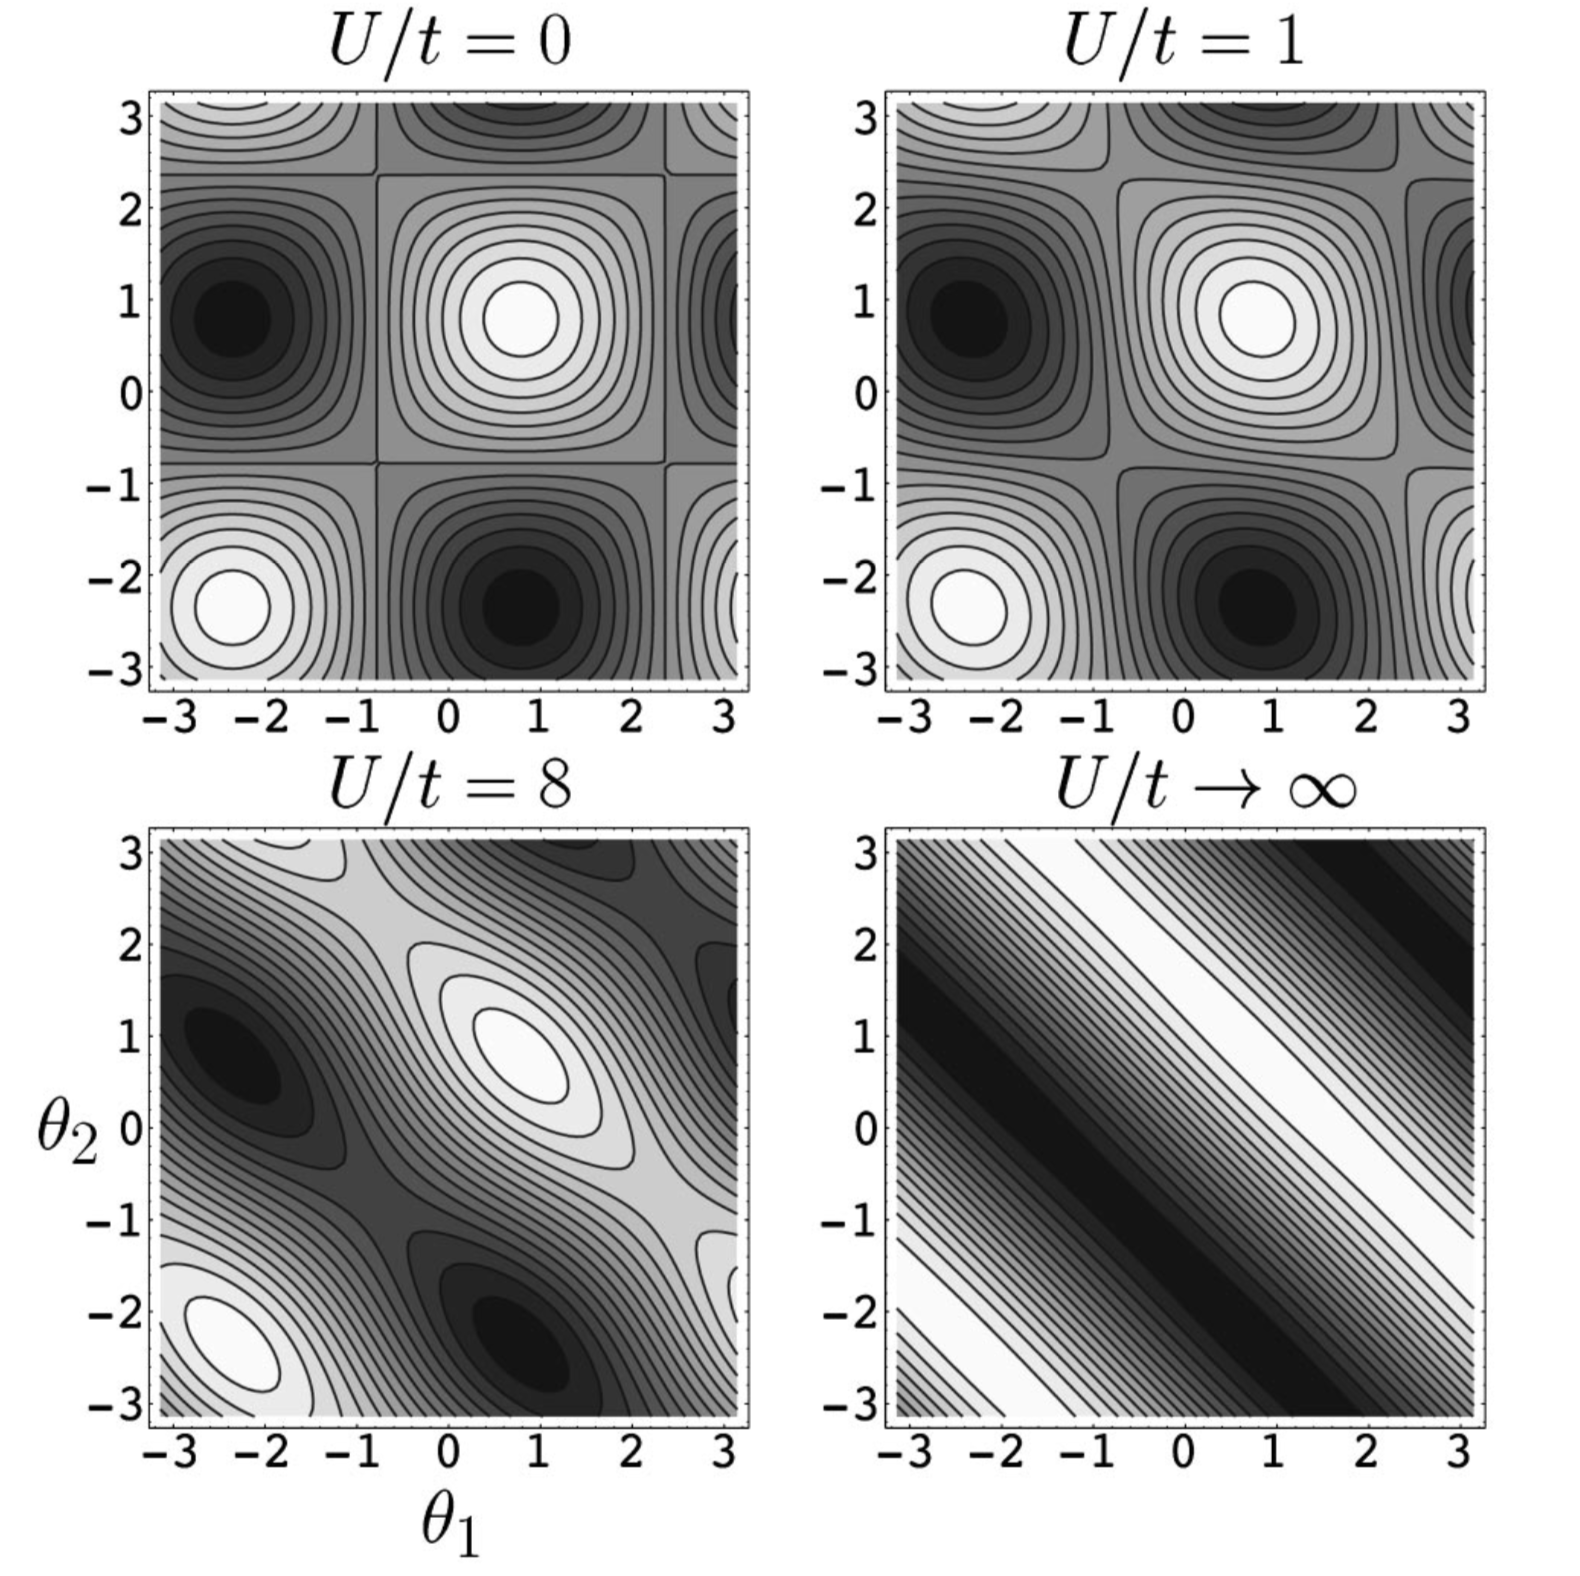
\includegraphics[width = 6cm]{Introduction/constrained.png}
\caption{ Contour plots of the two-fermion ground state wave function overlap $<\chi | \phi_0 >$ for a Hubbard model as obtained in \cite{constrained2}. The parameters $\theta_{1,2}$ arise from the decomposition $|\chi > = (\cos\theta_1 c_{1\uparrow}^\dagger + \sin\theta_1 c_{2\uparrow}^\dagger) (\cos\theta_2 c_{1\downarrow}^\dagger + \sin\theta_2 c_{2\downarrow}^\dagger)$, where $c^{(\dagger)}$ are annihilation (creation) operators of two fermions with either spin up or down. Notice the varying nodal surfaces as the interaction energy-hopping parameter ratio varies. The accuracy of the constrained path QMC method depends on the shape of these surfaces (taken from \cite{constrained2}). }
\end{figure}

\subsection{Determinantal/Auxiliary Field QMC}\paragraph{}

The idea of this method is establish a mapping between quantum and classical Monte Carlo, using a suitable change of variables. The random variables are then sampled from the configuration space of the corresponding classical problem. The price to pay is that for a d-dimensional quantum problem, the corresponding classical problem is $(d+1)$-dimensional: an additional degree of freedom is added, and as we will show it corresponds to an imaginary time.

The expected value of a physical observable $\mathcal{O}$ may be written as $<\mathcal{O}> = Tr (\mathcal{O}\mathcal{P})$, where we have defined a projection operator

\begin{equation}
\mathcal{P} = \frac{1}{\mathcal{Z}}e^{-\beta\mathcal{H}} \, , \mathcal{Z} = Tr (e^{-\beta \mathcal{H}}) = \sum_i < \psi_i | e^{-\beta \mathcal{H}} | \psi_i > ,
\end{equation}
and the trace is taken over the Hilbert space describing all possible occupations in a lattice model.\par

Finding an approximation to the projection operator which is amenable to computation is done in terms of the Hubbard-Stratonovich transformation: the problem is  reformulated in terms of auxiliary variables $h_i$. The set $\{h_i\}$ is known as the Hubbard-Stratonovich field.\par

In the end, we sample configurations, that is, particular realizations of the HS field, with probability $P(h)$. It is the computation of this probability that requires determinant calculations giving the name to the method. For concreteness, we state without proof that for the example of the Hubbard model we have:

\begin{equation}
P(h) = \frac{\eta_d}{Z_h} \det [ M_{+}(h) ] \det [ M_{-}(h) ] ,
\end{equation}
where $M_\sigma (h)$ are fermion matrices depending on the imaginary time frame, spin, and the HS field; $\eta_d$ is simply a normalization constant depending on dimension, and $Z_h$ is the partition function expressed in terms of the HS field \cite{qmc}.

To move from a configuration $\{h\}$ to a new one $\{h'\}$, we vary, or flip, the value of only one variable $h_i$, leaving the rest unchanged. We use an acceptance-rejection scheme - the Metropolis-Hastings algorithm - that ensures that the accepted sample configuration follows the desired distribution. Once we reach equilibrium, i.e. the Markov Chain hits the stationary distribution, we have finished the so called warm up steps, and we may start measuring.\par

Recall the reasoning that was made in section \ref{subsec:dmc}. The solution of the Schr\"odinger equation may be expressed in terms of a linear combination of stationary states, which depend on time via a factor $e^{-iE_n t}$, where $n$ labels the energy level of the quantum system under study. We choose the energy scale so that all energies are positive and perform a change of variable to imaginary time $t= -i\tau$. The solution's time dependence is now described by a sum of transients $e^{-E_n \tau}, \, n \in \mathbb{N}$, and by following the (imaginary) time evolution of the wave function long enough, we will asymptotically reach the ground state energy $E_0$, and its corresponding wave function $\phi_0$. Note that this is independent of the initial condition in which we prepare the system. Convergence speed may eventually depend on this choice, but from a mathematical point of view if we wait long enough only the ground state will survive. The imaginary time many-body propagator $U(\tau) = e^{-H\tau}$ filters a trial wave function $\phi$ to the exact ground state $\phi_0$:

\begin{equation}
E_0 = \lim_{\tau \rightarrow \infty} \frac{<\phi | HU(\tau) | \phi >}{<\phi | U(\tau) | \phi >}
\end{equation}

We impose the condition that $\phi$ mustn't be orthogonal to $\phi_0$. Additionally, we require $\phi$ to be a symmetrized (antisymmetrized) product of single-particle orbitals for bosons (fermions).\par

The method can be used to treat systems with a variety of interactions. In general:

\begin{equation}\label{eq:general_h}
\mathcal{H} = \sum_{\alpha\beta} K_{\alpha\beta} \rho_{\beta\alpha} +\frac{1}{2} \sum_{\alpha\beta\gamma\delta} v_{\alpha\beta\gamma\delta} \rho_{\gamma\alpha} \rho_{\delta\beta} ,
\end{equation}
where $\rho_{\beta\alpha}\equiv a_\alpha^\dagger a_\beta$ and
$K_{\alpha\beta} = T_{\alpha\beta} \pm \frac{1}{2} \sum_{\gamma} v_{\alpha\gamma\gamma\beta}$
is the kinetic energy $T$ plus a self-interaction term for bosons or fermions, respectively. The subscripts ${\alpha, \beta, \gamma, \delta}$ represent eventually present degrees of freedom: spin, isospin, etc., as well as spatial coordinates \cite{sugiyama}.\par

We introduce an auxiliary field $h$ that reduces the exponential of the two-body operator in equation (\ref{eq:general_h}) to a functional integral over an infinite set of exponentials of one-body operators. We then run Monte Carlo to approximate these integrals. A valuable property of AFQMC is that it properly treats fermions: the HS representation of the propagator affords a description in terms of single-particle exactly antisymmetrized wave functions. GFQMC and DQMC do not share this property.\par

The long time behavior of a trial state: $\lim_{\tau \rightarrow \infty } e^{-\tau (\mathcal{H} - \varepsilon_0)} |\psi_T > = | \phi_0 > < \phi_0 | \psi_T >$ may be mapped onto a stochastic process in the manifold of N-particle Slater determinants $\mathcal{D}(N)$ \cite{zhang}. The mapping to a stochastic process is made possible by the discretization

\begin{equation}
e^{-\tau (\mathcal{H} - \varepsilon_0)} = (e^{-\delta \tau ( \mathcal{H} - \varepsilon_0 ) })^n \quad \text{with} \quad \delta \tau = \frac{\tau}{n}
\end{equation}

The HS transformation is in fact an operator identity that allows the establishment of a formal correspondence between a system of interacting fermions and an ensemble of non interacting fermion systems coupled to fluctuating external potentials. This leads to a random walk representation of the imaginary time evolution.\par

A limitation of the straightforward numerical implementation of AFQMC is that it leads to an exponential increase in statistical errors with imaginary time. This is due to the appearance of random complex phases during the evolution. To solve this problem, S. Zhang introduced an importance sampling transformation guiding the random walk \cite{zphase}  . This is done by introducing shift parameters in terms of which we rewrite $e^{-n\delta \tau (\mathcal{H} - \varepsilon_0)} |\psi_T >$. These parameters are chosen to minimize fluctuations in the importance function to first order in $\delta \tau$.\par

The aim is to solve the sign problem which arises when the overlap between one or more walkers and the trial state vanishes, yielding large fluctuations in the importance function, and generating statistical errors in AFQMC's estimates.

\subsection{Computational Complexity and the Sign Problem}

The sign problem afflicting many-fermion QMC causes an exponential increase of the computing time with the number of particles. A polynomially scaling algorithm would provide an unbiased and numerically exact solution (as in the case of bosons) for the problem of simulating a strongly correlated electron system. However, the problem was recently shown to be NP hard \cite{troyer}. Solving the sign problem would solve all NP problems in polynomial time (proving that $NP = P$) in what would be a major breakthrough in mathematics. This is widely believed to be unlikely, i.e. there is a conjecture that $NP \neq P$, although currently no mathematical proof exists of this impossibility.\par

Specific sign problems might be solvable. This indeed happens for a restricted subclass of quantum systems, for example see \cite{wiese, arnow,kalos}. An interesting open question is that of determining which models allow a partial solution of the sign problem due to their special properties. In particular, it is relevant for this field whether the 2D fermionic Hubbard model belongs to this class or not. A promising idea to circumvent NP hardness is to use ultracold atoms in optical lattices \cite{optical}, effectively using a quantum simulator to study the phase diagrams of correlated quantum systems. Although promising, even this method may not solve the problem in general: it is also still an open question whether a quantum computer could ever solve the NP complete problem (see \cite{troyer} and references therein).